\chapter{Judges and Officials Rules}

\section{Standard Skill Officials}%comment-2016 this should be fixed so it only applies to standard skills
\oldrule{1.29}
\textbf{Artistic Director:} The head organizer and administrator of artistic events.
The Artistic Director's job starts well before the convention, arranging equipment for the gyms (or performing areas) and recruiting the other artistic officials.
With the Convention Host, the Artistic Director determines the operating systems, paperwork and methods to be used to run the events.
With the Chief Judge, the Artistic Director is in charge of keeping events running on schedule, and answers all questions not pertaining to rules and judging.
The Artistic Director is the highest authority on everything to do with the artistic events, except for decisions on rules and results.

\textbf{Chief Judge:} Like the Referee, the Chief Judge should be a thoroughly experienced person who must above all be objective and favor neither local, nor outside riders.
The Chief Judge must be thoroughly familiar with all of the artistic officials' jobs and all aspects of artistic rules.
The Chief Judge oversees everything, deals with protests, and answers all rules and judging questions.
The Chief Judge is responsible for seeing that all artistic officials are trained and ready, and that the artistic riding areas are correctly measured and marked on the floor.
The Chief Judge is also responsible for the accuracy of all judging point tabulations and calculations.

\section{Training Officials}
\oldrule{1.20}
As the rules state, competitions cannot be started until all key artistic officials have been trained and understand their tasks.
For Artistic events, the Chief Judge is in charge.
For certain artistic events, a minimum level of judging experience is required.
See section \ref{sec:freestyle_judging-panel}.

\section{Interruption Of Judging}
\oldrule{6.6}
An interruption of judging can result from material damage, injury or sudden illness of a competitor, or interference with a competitor by a person or object.
If this happens, the Chief Judge determines the amount of time left and whether any damage may be the fault of the competitor.
Re-admittance into competition must happen within the regulatory competition time.
If a routine is continued and the competitor was not at fault for the interruption, all devaluations coming forth from the interruption will be withdrawn.

\section{Competitor and Judging Forms}
\oldrule{6.41.4}

If available to the organizers, a computer database should be used to generate forms for both the competitor and the judges, and then be used to calculate the scores.
Either the Writing Judge Form or the traditional Standard Skill Form is required for judging.
The other forms are suggested to help both the competitors and judges.
Suggested forms are: 
\begin{itemize}
\item \textbf{Competitor Form:} Skill Order, Figure number and letter, Description, Score, and Skill Definition.
\item \textbf{Standard Skill Form:} Skill Order, Figure number and letter, Description, Score, and areas to mark 50/100\% technical devaluations and the ~ / + 0 execution devaluations.
An area at the bottom should be included to write in the names of the three judges.
An area at the bottom should also be included to help in manual scoring of the routines.
\item \textbf{Writing Judge Form:} Skill Order, Figure number and letter, Description, Score, and areas to mark 50/100\% technical devaluations and the ~ / + 0 execution devaluations.
An area at the bottom should be included to write in the names of the three judges.
\item \textbf{Difficulty Judge Form:} Skill Order, Figure number and letter, Description, Score, Skill Definition, and area to mark 50/100\% technical devaluations.
The addition of the Skill Definition can help the judge if there is clarification needed for the correct execution of the skill.
\item \textbf{Execution Judge Form:} Skill Order, Figure number and letter, Description, Score, and area to mark the ~ / + 0 execution devaluations.
\end{itemize}

All three judging forms should have gray shading to indicate the relative speed of the skills.
No shading would indicate a slower skill (typically all riding skills), a light gray indicates skills that are quicker than the riding skills (most of the counted short skills), and a dark gray indicates skills that are very quick.
This will help the judges estimate how quickly they must watch for new skills.

\section{Judging Panel \label{sec:freestyle_std-judging-panel}}
\oldrule{6.42}
There will be 1 Chief Judge, 2 Difficulty Judges, 2 Execution Judges, 2 Writing Judges, and 1 Timer.
The judging panel will be divided into two judging units, each consisting of one Difficulty, one Execution, and one Writing Judge.
The judges will be appointed to the functions Writer, Execution, and Difficulty, respectively in order of their experience.
At Unicons, all judges for the Expert groups must have previous Unicon judging experience.

\section{Operation Of The Judges}
\oldrule{6.43}
While the Difficulty and Execution Judges watch the routine, the Writing Judge reads the names of the figures from the list.
The Difficulty Judge indicates if a skill was fully completed, or the reduction percentage if it was not.
The Execution Judge indicates the execution mistakes using symbols, as described below.
The Writer writes down the verbal remarks of both judges on the judging sheet.
For this reason, the Writer is seated between the other two judges.
The position of the judging table must be so that all judges have a clear view of the entire riding area.
There must be enough space between the two judging units to ensure their working independently of each other.

A video of the performance may be reviewed if there are discrepancies in judge scores, or if a judge is in doubt about one or more of his/her scores.
When time allows, video can be reviewed by approval of the Chief Judge.
The Chief Judge should prearrange for routines to be recorded, but this is not a mandatory requirement.

Alternatively, to speed up the competition and judging, video cameras should be used to record the competition.
There must be at least two cameras, one on each of the two corners.
A third camera in the center is also good for a backup.
The recordings should be downloaded to a computer in approximately groups of ten competitors.
The judges will all be in a separate viewing area to watch the videos and make their scores.

\section{Difficulty Devaluations}

\subsection{Skill Verification}
\oldrule{6.44.1}
Every figure on the judging sheet must be executed according to its description in the Standard Skill List.
If a performed figure does not correspond with the entry on the judging sheet, 100\% is devaluated.

\subsection{Technical Mistakes}
\oldrule{6.44.2}
If a technical mistake occurs during the execution of a skill, 50\% is devaluated.
Technical mistakes include but are not limited to the following: 
\begin{itemize}
\item Part of body other than one hand touching seat in seat out skills
\item Hand holding seat touching body in seat out skills
\item Free foot touching rotating part of unicycle in one foot skills
\item Legs not extended and/or toe not pointed for skills where the leg is quickly extended (including, but not limited to: wheel grab, crank idle kick, hop on wheel kick)
\end{itemize}

\subsection{Skill Completion \label{subsec:freestyle_difficulty-devaluations_skill-completion}}
\oldrule{6.44.3}
Every figure on the judging sheet must be performed as entered, from start to finish, without the rider touching the floor, except where required to by the figure description.
This applies to all skills: riding skills (figures in lines, circles and 8's), transitions, axis skills, single and counted short skills, and mounts.

\begin{wrapfigure}{l}{0.35\textwidth}
\vspace{-25pt}
\begin{center}
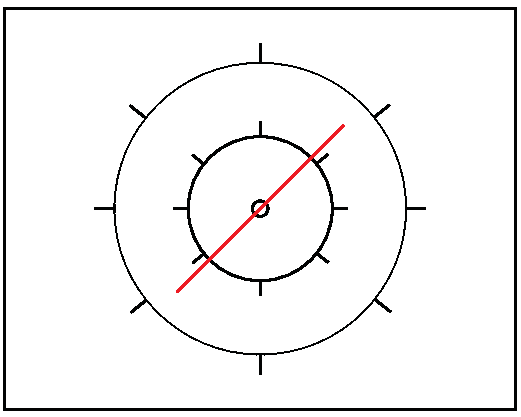
\includegraphics[width=0.33\textwidth]{std_skill_error_1}
\end{center}
\vspace{-20pt}
\caption{50\% Devaluation \label{fig:std_skill_error_1}}
\vspace{-5pt}
\begin{center}
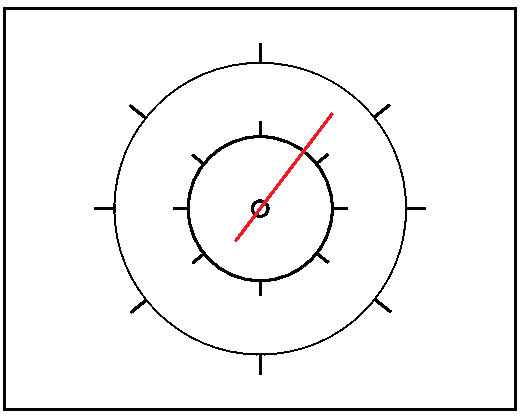
\includegraphics[width=0.33\textwidth]{std_skill_error_2}
\end{center}
\vspace{-20pt}
\caption{100\% Devaluation\label{fig:std_skill_error_2}}
\vspace{-25pt}
\end{wrapfigure}

\textbf{Riding Skills, Repetitive Axis Skills, and Counted Short Skills:} If a figure is broken off in the first half of its required execution, or performed for less than half of the required execution, 100\% is devaluated.
If a figure is broken off in the second half of the required execution, or performed for less than the required execution, 50\% is devaluated.

\textbf{Riding Skills:}
If a rider is not in position for a line figure before crossing the 8-meter circle, but is in position when crossing both 4-meter circle lines, 50\% is devaluated (see figure \ref{fig:std_skill_error_1}).
If the rider is in position but only crosses one edge of the 4-meter circle, 100\% is devaluated (see figure \ref{fig:std_skill_error_2}).

\textbf{Transitions and mounts:} Must finish in the end position (one revolution, $2 \frac{1}{2}$ hops, or $2 \frac{1}{2}$ idles) or 100\% is devaluated.
If the end position for a mount is not defined, must perform one revolution, OR $2 \frac{1}{2}$ hops, OR $2 \frac{1}{2}$ idles before stepping off the unicycle.

\textbf{Axis skills:} If the end position for a axis skill is not defined, must perform one revolution before stepping off the unicycle.
The ending position is not required to be the same as the starting position.

\textbf{Single Short Skills:} Unless otherwise defined in the skill description, the ending position is the same as the starting position.
Must finish in the end position (one revolution, $2 \frac{1}{2}$ hops, or $2 \frac{1}{2}$ idles) or 100\% is devaluated.
If the start and end position for a single short skill is not defined, must perform one revolution, $2 \frac{1}{2}$ hops, OR $2 \frac{1}{2}$ idles before stepping off the unicycle.

\subsection{Start Of Figures}
\oldrule{6.44.4}

All figures start when the rider gets into the position required for that figure.

\subsection{Figure Order}
\oldrule{6.44.5}

Figures left out according to their order on the judging sheet are devaluated 100\%.
This devaluation remains, even if the figure is performed afterward.

\subsection{Figure Patterns}
\oldrule{6.44.6}

Riding figures that the rider doesn't attempt to be ridden as described in section \ref{subsec:freestyle_floor-markings-figure-shapes_riding-area-boundaries} should receive 100\% devaluation.

\textbf{Example:} The line figure is described as ``…start outside the large (8m) circle, cross the center circle, and continue outside the large circle''.
If the rider does not attempt to cross the center circle and performs the line circle completely outside the 4m circle, then 100\% is devaluated.

\section{Execution Devaluations}

\subsection{Wave (\textasciitilde) = -0.5 Point}
\oldrule{6.45.1}

A wave is scored once per skill for each of the following execution mistakes listed below.
More than one wave can be applied to each skill, but if a rider makes the same mistake twice during one skill, they should only receive one wave.

\textbf{Example:} During wheel walking, a rider may have jerky body movements and fingers not together at the beginning – two waves should be applied.
If the rider then smoothly wheel walks for a while and then has jerky body movements again, a third wave should not be applied.
\begin{itemize}
\item insecure entrance or exit 
\item cramped, insecure execution 
\item jerky body movements 
\item not sitting up straight 
\item fingers not together 
\item free leg not stretched, toes not pointed 
\item waving arms 
\item jerky pedal movement 
\item line not straight 
\item circle not round 
\item crossing the 4 m circle when performing a skill in a circle 
\item failure to cross center circle in line or figure 8 
\item circles of figure 8 not the same size 
\item pedal, or foot on pedal touching floor 
\item wandering spin or pirouette 
\item circle size exceeds 1 meter diameter in a spin 
\item going outside riding area boundary 
\item looking at the standard skill order 
\item arms not stretched 
\item arms not horizontal 
\item palms not down 
\item arms touching the body during seat out skills
\end{itemize}

\subsection{Line (/) = - 1 Point}
\oldrule{6.45.2}

A line is scored every time loss of control occurs.
Loss of control includes:
\begin{itemize}
\item loss of proper body form 
\item breaking off and restarting a skill 
\item loss of proper body form before or after transitions
\end{itemize}

\subsection{Cross (+) = - 2 Points}
\oldrule{6.45.3}

A cross is scored each time an unintentional dismount occurs with the competitor landing on his or her feet without the unicycle being dropped.

\subsection{Circle (0) = - 3 Points}
\oldrule{5.41.4}

A circle is scored each time an unintentional dismount occurs with a part of the rider other than his or her feet touching the floor (hand, knee, rear, etc.) or with the unicycle being dropped.
Seat drag skills only have this score applied if a part of the rider other than the feet touches the floor.

\subsection{Applying Lines, Circles, Crosses}
\oldrule{6.45.5}

Lines, circles and crosses are scored every time they occur during and between all skills, whether entered on the score sheet or not.
Only the highest applicable devaluation symbol shall be imposed per execution mistake.
Most waves are not scored if they occur between skills listed on the judging sheet.
Waves can only be scored between skills if they are unrelated to body form.

\textbf{Example:} A competitor will not get a wave if the competitor's arms are not in proper form between skills listed on the judging sheet, but a competitor will get a wave for exceeding the riding area boundary.

\section{Totaling Scores}
\oldrule{6.46}
After the routine is finished, the percentages and symbols from the judges are converted into numbers.
These numbers are subtracted from the rider's starting score.
Then, the scores of the two judging units are added together and divided by two to get the finishing score of a competitor.
The winner in the Standard Skill event is the competitor with the highest score.
If more than one competitor have the same score, placing is decided by the highest Execution score.
If those scores are also the same, the competitors receive tie scores.
